%!TEX root = *.tex
%%%%%%%%%%%%%%%%%%
% カウンタのリセット
\setcounter{figure}{0}
% 問題文
一様な材質でできた薄い剛体円板の水平面上での運動を考えよう.
本問を通して,摩擦や空気抵抗はすべて無視する.
したがって,円板は並進運動のみを行い,回転することはない.

\begin{enumerate}[\ajRoman{\arabic{enumi}}]
  \setlength{\leftskip}{-1zw}
  \setlength{\itemindent}{1zw}\setlength{\labelsep}{0.5zw}
  \setlength{\labelwidth}{1zw}\setlength{\leftmargin}{1zw}
  \setlength{\itemsep}{0.5\baselineskip}
  \item 図1のように,質量が$m,\,M$で同じ大きさの2つの剛体円板の間に,ばね定数が$k$である厚みと質量の無視できるばねをはさみ,両側から力を加えてばねを$l$だけ縮ませた状態で,なめらかな水平面上に固定する.その後静かに固定を解いた.ばねの長さが自然長に戻ったときの質量$m$の円板の速さ$v$を$k,l,m,M$を用いて表せ.
  \begin{figure}[H]
    \centering
    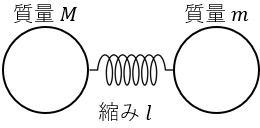
\includegraphics[width=.3\columnwidth]{../graphs/open_19_8_1-1.png}
    \caption{}
  \end{figure}
  \item 質量が$m_{\rm A},\,m_{\rm B}$の剛体円板がA,Bがある.静止しているBに速さ$v_0$でAが衝突した結果,それぞれの速さは$v_{\rm A},\,v_{\rm B}$となり,
  それぞれの速度の向きはAの入射方向に対して$\theta,\,\phi$となった.
  ここで図2のようにAの入射方向に\x 軸,それと垂直な方向に\y 軸をとる.
  \begin{enumerate}[(1)]
    \setlength{\leftskip}{-2zw}
    \setlength{\itemindent}{1zw}\setlength{\labelsep}{1zw}
    \setlength{\labelwidth}{1zw}
    \item 衝突前後の運動量保存則の式を,\x 軸方向と\y 軸方向に分けて書け.
    \item 2つの剛体円板の大きさを無視し,はじめにBが静止していた位置を原点とし,$m_{\rm A}=m_{\rm B}$とする.このとき,衝突後の角度が$\theta=30^\circ,\,\phi=60^\circ$になった.Aが座標$(9,\,3\sqrt{3})$に達したとき,Bが達する点の座標を求めよ.
  \end{enumerate}
  \begin{figure}[H]
    \centering
    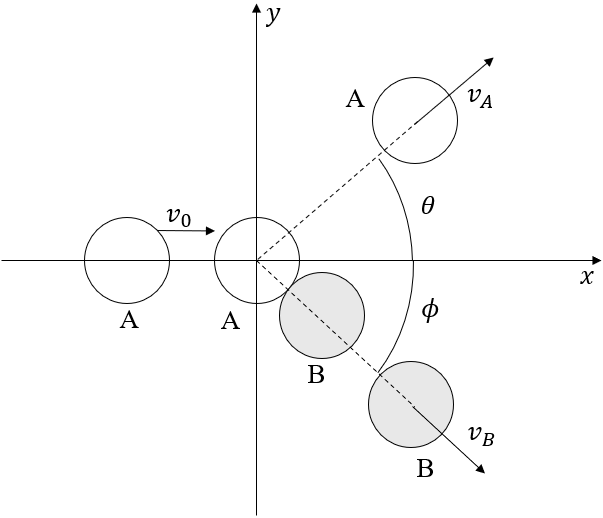
\includegraphics[width=.55\columnwidth]{../graphs/open_19_8_1-2.png}
    \caption{}
  \end{figure}
  \item 同じ半径で同じ質量$m$の4つの剛体円板1,2,3,4を,図3のように水平面上に配置して静止させる.円板1と4の中心を結ぶ直線を\x 軸とし,それと垂直な方向\y 軸をとる.まず,\x 軸負の方向から4つの円板と同じ質量で同じ半径の剛体円板0を速さ$u_0$で衝突させる.その後の様子を次の3段階に分けて考えてみよう.ただし,それぞれの衝突はすべて弾性衝突であるとする.
  \begin{enumerate}[(\ajroman{\arabic{enumii}})]
    \setlength{\leftskip}{0zw}
    \setlength{\itemindent}{1zw}\setlength{\labelsep}{1zw}
    \setlength{\labelwidth}{1zw}
    \item 剛体円板0と1の衝突
    \item 剛体円板1と2,1と3の同時衝突
    \item 剛体円板2と4,3と4の同時衝突
  \end{enumerate}
  \begin{enumerate}[(1)]
    \setlength{\leftskip}{-2zw}
    \setlength{\itemindent}{1zw}\setlength{\labelsep}{1zw}
    \setlength{\labelwidth}{1zw}
    \item (\ajroman{\arabic{enumii}})の衝突直後の剛体円板1の速さ$u_1$を求めよ.ここではまだ,剛体円板1は2,3と衝突していないものとする.
    \item 次に(\ajroman{\arabic{enumii}})の衝突を考える.ここではまだ,剛体円板2,3は4と衝突していないものとする.円板2には1からの力積のみが作用するので,衝突直後,その速度の向きは円板1,2の中心を結ぶ直線に沿った向きとなる.衝突直後の円板1の速度の\x 成分を$v_1$,円板2の速さを$u_2$とする.対称性より,円板2と3の速度は\x 軸に関して対称でその速さは等しくなることに注意して,速さの比$\dfrac{\abs{v_1}}{u_1},\,\dfrac{u_2}{u_1}$をそれぞれ求めよ.
    \item (\ajroman{\arabic{enumii}})の衝突直後の剛体円板2,4の速さをそれぞれ$v_2,\,v_4$とし,また,2の速度の向きと\x 軸の向きとのなす角度を$\theta_2$とする.速さの比$\dfrac{v_2}{u_2}$と$\dfrac{v_4}{u_2}$,および$\tan{\theta_2}$の値をそれぞれ求めよ.
    \item すべての衝突が終わった後の剛体円板1の速度を$w_1$とするとき,速さの比$\dfrac{\abs{w_1}}{u_2}$を求めよ.
  \end{enumerate}
  \begin{figure}[H]
    \centering
    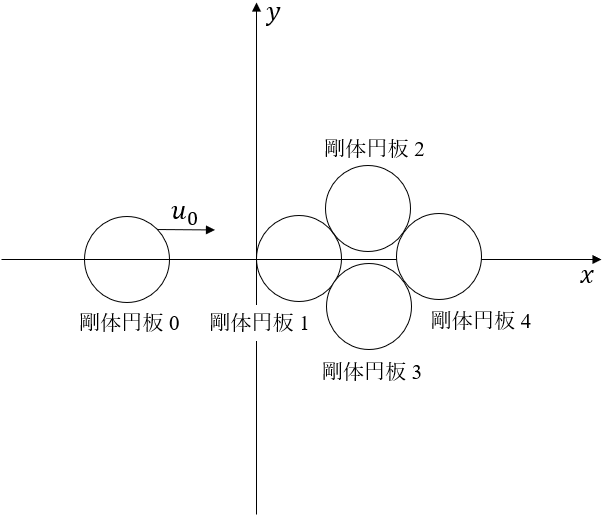
\includegraphics[width=.55\columnwidth]{../graphs/open_19_8_1-3.png}
    \caption{}
  \end{figure}
\end{enumerate}



%%%%%%%%%%%%%%%%%%